\chapter{Telemanipulátor programja}
\label{sec:Prog_nagy_fej}

A telemanipulátor jelfeldolgozó rendszerének fizikai összeállítása után a szenzorok által küldött jelek szoftveres feldolgozását és használatát mutatom be. A fejezet során hasonlóan mint korábban a szenzoroktól kezdem a szoftveres komponensek bemutatását és haladok a tényleges robotkar mozgatásra szolgáló rendszerekig.

%----------------------------------------------------------------------------
\section{Szenzor kommunikációs protokollja}
\label{sec:ssc_kom}
%----------------------------------------------------------------------------
A GMR szenzor a mikrovezérlővel az úgynevezett Synchronous Serial Communication\footnote{magyarul Szinkron Szériás Kommunikációs} röviden SSC protokollt használ. Ez a protokoll egy olyan kommunikációs csatorna, amely során a küldő és a fogadó eszközök szinkronizáltak egymással a közös órajel alapján. Az SSC azon alapul, hogy mindkét eszköz előre rögzített órajelet használ a bekapcsolás pillanatától, hogy a rendszer használ teljes ideje alatt szinkronban maradjanak.

A protokollon közös órajele biztosítja, hogy az adat transzferálás esetén mindkét eszköz azonos sebességgel és időzítéssel küldje és fogadja az üzenetet. Ez az információ küldés során bitek sorozataként továbbítódik, és a kommunikációban résztvevő fogadó és küldő egységek egyeztetik az adatok kezdőpontját és végpontját az órajelet és a protokoll definícióit használva. Ennek következtében mindkét eszköz tudja, hogy mikortól kell és meddig értelmeznie az érkező biteket.

%TODO kép a GMR bitekről

A protokoll lehetővé teszi a teljes és a half-duplex kommunikációt. Teljes-duplex esetén mindkét eszköz képes egyszerre küldeni és fogadni adatokat, míg half-duplex esetén a kommunikáció váltakozva történik, azaz egyik eszköz küld, majd vált, és a másik eszközről fogad.

Az SSC gyakran használt alkalmazása az I2C (Inter-Integrated Circuit) és a SPI (Serial Peripheral Interface) kommunikációs protokollok. Az I2C esetén a kommunikáció két vezetéken, az egyiken az adat másikon pedig az órajel jelzés  történik, míg az SPI esetén több vezetéket használhatunk, például MISO (Master In Slave Out), MOSI (Master Out Slave In), órajeladóval és cél választóvonallal.

Az SSC protokoll széles körben alkalmazható az elektronikában és a beágyazott rendszerekben, ahol szükség van a gyors, megbízható és szinkronizált adatkommunikációra a különböző eszközök között.

A telemanipulátor esetében half-duplex kommunikációs protokoll beállítási módot használok a GMR szenzor dokumentációjában\footnote{\ref{sec:melleklet} melléklet TLE5012B dokumentum alapján} meghatározott követelmények szerint. Minden szenzorhoz tartozóan chipválasztó pineket is deklarálnom kellett. A kommunikációs protokoll kezeléséhez egy előre elkészített könyvtárat használtam, ami megtalálható a (\ref{sec:melleklet}.melléklet) mellékletben.

\section{Mikrovezérlő program}
\label{sec:MCU_program}
%----------------------------------------------------------------------------

A mikrovezérlő program a diploma dolgozathoz képest kisebb módosításokkal lett kiegészítve, de igazán nagy fejlesztést nem igényelt. Az elvárásoknál támasztott követelményeknek megfelelt, kellően gyors és könnyen módosítható lett. Erről részletesebben a \ref{sec:ujratervezesi_szempontok}.fejezetben beszámoltam.

A telemanipulátornál használt program a konzulensem által készített hasonló elven működő haptikus vezérlőjének(\ref{sec:melleklet}.melléklet) a mikrovezérlő programját vettem alapul. A programot a saját eszközömhöz szükséges módosításokkal elláttam, mivel ez is STM32-es fejlesztőkörnyezetben lett készítve.

Fő különbségek, hogy a mikrovezérlő az én általam használt telemanipulátor esetében $7[db]$ szenzor adatait gyűjti össze, dolgozza fel és továbbítja a további rendszereknek.

A mikrovezérlő programba implementált funkciók a következők:

\begin{itemize}
\item Szögérték kiolvasás
\item Szögérték offszetelés
\item Szögérték kinemtaikailag felvett forgás tengelyre igazítása
\item Szögértékek tömbértékek összegyűjtése
\item Kommunikáció a mikrovezérlőhöz csatlakoztatott számítógéppel
\end{itemize}

A szögértékeket szekvenciálisan az $1.$ csukló szenzortól a $7.$ csukló szenzorig egymás után olvassa ki. A szenzor kommunikáció már a bemutatott SSC kommunikáción történik és minden szenzor saját chipselect pin-jének a jelváltozására\footnote{A TLE 5012B GMR szenzor esetében alacsony jelről magas jelre vált a kommunikáció alatt} történik. A kiolvasott szögérték a szenzor meghatározott egyik tengelye és a mágnes kétpólusa által megadott póluspárok egymással bezárt szöge.

%TODO Kép a szenzor szögről.

Ez a megkapott szögérték $-180^\circ$ és $180^\circ$ állású közötti lehet. Ezt az értéket én átkonvertáltam $0^\circ$ és $360^\circ$-os skálára ugyan is így sokkal könnyebben beállítható az offset és a forgás irány is egyértelműbb számomra. Az offszet paraméterek beállítása a program indulása után is változtatható, de az alapparaméterek be vannak égetve. Az oka ennek, hogy így nem kellett minden tesztelési ciklus elején offszetelnem csuklóban lévő szenzorokat. Az offszet értékeket a következőképpen állapítottam meg.

\begin{enumerate}
  \item Minden csuklón van egy jelző egyenes, ami a két tengely koordináta rendszereinek a párhuzamosságát jelenti abban az állásban
  \item A kinematikai felírásban vett koordináta rendszer szerinti nullába mozgattam a megfelelő csuklót
  \item Kiolvastam a szenzor adott csuklóhoz tartozó értékét
  \item Az előzőpont alapján, ha pozitív előjelű volt akkor kivontam, ha pedig negatív akkor hozzáadtam a kiolvasott értékhez az offszetet
\end{enumerate}

Az így megkapott szögértékek elfordulására kell még figyelni. Ugyanis a szenzor és mágnes elhelyezkedése a tengelyen befolyásolja, hogy a szögérték a tengely körüli elfordulással melyik irányba pozitív. Ha a forgatási irány eltér, egyszerűen a szögérték mínusz egyszeresét kell venni. 

Ezt követően, ha minden szögértéket továbbítja a mikrovezérlő, ha igény van rá. Az igényt az számítógépen futó interface támasztja még pedig, az UART porton küldött üzenettel. A jelenleg implementált parancsok:

\begin{itemize}
\item $RDS$ - Read from sensor - Szenzor értékek kiolvasás 
\item $KA$ - Keep Alive - Kapcsolat fenntartására vonatkozó parancs
\item $REC$ - Read Error Counter - Hibás kiolvasások darabszámának kiolvasása
\item $CEC$ - Clear Error Counter - Hibás kiolvasás számláló törlése
\end{itemize}

A fenti parancsok közül a REC, CEC és a RDS parancsokat használom. Az RDS esetén a szögértékek kiolvasásra kerülnek és továbbítódnak UART porton, ahogy listában említettem. A továbbítás egy nagy méretű byte tömbben történik, aminek az első két érték amit továbbít egy "OK" és maga az RDS paranccsal megkapott üzenet, a többi érték a szenzorokból kiolvasott és számított szögértékek. A REC és a CEC parancsot a szenzorok üzembe helyezésekor használtam. Egy egyszerű port terminál kezelését lehetővé tévő programmal csatlakoztam a mikrovezérlőre és elküldtem a RDS parancsot, kétszer. A két kiadott parancs között megváltoztattam a telemanipulátor orientációját és ha a szögérték változott a szenzort mműködőnek tekintettem. A beüzemelés alatt, több szenzor se működött azonnal, és a CEC és REC parancsokkal tudtam a hiba darabszám tárolókat kiolvasni és törölni. A továbbiakban szeretnék még offszet érték beállítására vonatkozó metódust implementálni, illetve jelrögzítést és offszet-be állásra vonatkozó parancsokat.

A mikrovezérlő programmal kapcsolatban nagyon fontos még kitérni a RTOS rendszerre. Ez a STM32 vezérlőknél elérhető funkció a valós idejű lefutáshoz nagyon közeli működést tesz lehetővé. A program így előre megjósolható és determinisztikus módon válaszol az eseményekre, ugyanis realtime rendszerekben a feladatoknak szigorú időkorlátoknak kell megfelelniük, és az RTOS biztosítja a prioritáskezelést, időosztást és egyéb funkciókat a hatékony valós idejű működés érdekében.

%TODO rtos kép
%TODO RTOS HOL?????

A kritériumokban(\ref{sec:ujratervezesi_szempontok}.fejezet) meghatározott $4[ms]$ vagy gyorsabb lefutás a robot vezérlés eléréséhez nagyban hozzájárul ez a lehetőség. A RTOS-sel elérhető párhuzamos lefutószerű működés és a szigorúan definiált feladatok, a mikrovezérlő szögérték kiolvasási feladatát biztosítja, hogy megfeleljen a kritériumoknak.

\subsection{UART port}
\label{sec:uart_port}

%TODO UART port
%----------------------------------------------------------------------------
Az "UART" rövidítés a "Universal Asynchronous Receiver/Transmitter" kifejezést takarja. Ez a port egy soros kommunikációs protokoll, amely a digitális adatok átvitelét teszi lehetővé két eszköz között. Ez a protokoll olyan eszközök közötti soros kommunikációt biztosít, amelyek között nincs központi órajel (asynchronous), tehát az adatküldés és fogadás időzítése a két eszköz között előre nem definiált.

Az UART általában két vezetéken keresztül történik, amiket TX (Transmitter) és RX (Receiver) vezetéknek nevezünk. Az adatok a TX vezetéken keresztül mennek egyik eszköztől a másikig, és az RX vezetéken keresztül az ellenkező irányba. A kommunikációt start és stop bitek, valamint adatbitek alkotják.

Ez az interfész  vagy kommunikációs port a hardver vagy a vezérlő, amely lehetővé teszi az UART protokollt támogató eszközök közötti kommunikációt. Az UART portok széles körben alkalmazottak, például számítógépek, mikrovezérlők, beágyazott rendszerek és egyéb eszközök kapcsolódási pontjaiként. Segítségével a különböző eszközök adatokat küldhetnek és fogadhatnak egymástól.

\section{Haptikus interfész}
%----------------------------------------------------------------------------

A mikrovezérlő a számítógéphez, amin ez az interface fut UART porton(\ref{sec:uart_port}.fejezet) csatlakozik. A telemanipulátor csuklóiban mért szenzor jeleket a haptikus interface kéri el a mikrovezérlőtől. A haptikus jelző ebben az esetben azt jelenti, hogy visszajelzés is van építve a rendszerbe. A robotkar sikeres megfogás vagy ütközés esetén a haptikus interface képes az openmanipulátor (\ref{sec:melleklet}.melléklet) vezérlő telemnanipulátorába épített rezgő motoroknak jelet adni. Az általam készített telemanipulátorban nincs ilyen típusú visszajelzés beépítve. Az interface ezt a visszajelzési visszacsatolást leszámítva tökéletesen megfelel az általam kitűzött célnak. Ezt a szoftveres megoldást annak ellenére, hogy nem egy az egyben a saját munkám fontosnak tartom bemutatni, hogy a továbbfejlesztési lehetőségeknél ki tudjak arra térni, hogy miért lenne fontos ezt az eszköz interfacet tovább módosítani és fejleszteni.

Az interface két részre bontható. Az első az, ami megvalósítja a kommunikációt a mikrovezérlővel, a másik pedig egy ROS node, ami a telemanipulátorból kiolvasott szögjeleket publikálja.

Fontos megjegyezni, hogy a teljes dolgozatom Ubuntu vagy közismertebb nevén Linux operációs rendszeren lett megvalósítva. Windows operációs rendszeren is van lehetőség futtatni a programokat, de ebben az esetben viszont virtuális gépet\footnote{Olyan programok amelyek képesek Windows operációs rendszeren telepített programban valamilyen nem Windows környezetre készített programot futtatni} vagy Windows Subsystem for Linux\footnote{Microsoft által támogatott virtuális Linux operációs rendszer. Az egyik legelterjedtebb megoldás arra, hogy a Windows operációs rendszerrel rendelkező eszközökön a Linux-ot futassunk} - rövidítve WSL - kell használni. Természetesen számos más megoldás is van, mint például a dual-Boot\footnote{Linux és Windows operációs rendszerek ugyanazon eszközön egymás mellé a háttértárba fel vannak telepítve, és a számítógép elindulásánál lehet megválasztani, hogy melyiket akarjuk indítani. Ebben az esetben sokkal kiegyensúlyozottabb hardver terhelést kapunk és teljes értékű operációs rendszerekkel dolgozunk.}. Én a diploma dolgozatomban bemutatott telemanipulátor esetében teljes értékű Linux operációs rendszerrel ellátott, illetve dual-Bootos számítógépet használtam.

Az mikrovezérlővel a kommunikáció szerial kommunikáció, egy egyszerű USB-s csatlakozásnak minősül, ami azt jelenti, hogy lehetőség van információt küldeni és kiolvasni a port-ról. A csatlakoztatott mikrovezérlő a fizikai porton jelenik meg a számítógép port listájában (Linuxon ez a $tty*$ portok között van). A fizikai szerial kommunikáció létrejötte utána az interfacenek ugyanazok a kommunikációs paraméterek lettek beállítva, mint amit a mikrovezérlő is használ. Ez triviális ugyanis, ahogy a \ref{sec:MCU_program}.fejezetben bemutattam a UART protokollt fontos, hogy a két eszköz szinkronban legyen. A beállított paraméterek:

\begin{itemize}
\item Baudrate (Kommunikáció sebessége) - $115200 [-]$
\item Paritás Bit (Hibajelző bit) - Nincs
\item Stop bit szám - $1 [db]$
\item Byte méret - $8[db]$
\end{itemize}

Ezzel létrejött a programban is használható kommunikációs kapcsolat a számítógép és a mikrovezérlő között. Az interface ezt követően ciklikusan $8[ms]$-onként a kommunikációs porton az RDS parancs segítségével lekérdezi a csuklószögeket. A visszakapott választ ellenőrzi, hogy az előző fejezetben bemutatott sorrendben minden rendben megérkezik-e és így validálva az adatok helyességét. A megkapott csukló szögeket átváltja radiánba és a ROS topológián (\ref{sec:melleklet}.melléklet) is láthatóan publikálja őket.

\subsection{Robot Operating System - ROS}
%----------------------------------------------------------------------------
A Robot Operating System, röviden ROS, egy nyílt forráskódú, rugalmas és modularitásra épített szoftverrendszer, amelyet a robotok fejlesztéséhez és irányításához használnak. A ROS rendszerben minden önálló rendszereket node-oknak nevezzük. A node-ok egymással topic-okon keresztül tudnak kommunikálni.

Jobban megfogalmazhatóan a ROS egy gráfalapú rendszer, amelyben a különböző node-okat összekapcsolhatjuk egymással, hogy információt és parancsokat cseréljenek, komplex feladatok megoldása érdekében. A node-ok önálló egységek, amelyeket egymástól függetlenül fejleszthetünk és futtathatunk. Minden node specifikus feladatokat lát el, például szenzoradatok gyűjt (haptic interface), adatfeldolgozást végez (MoveIt) vagy irányítás vagy parancs kiadást hajt végre.

A node-ok közötti kommunikáció a már említett topic-okon keresztül történik. A topic egy adatcsatornának tekinthető, amely lehetővé az aszinkron adat közlést. Egy node publikálhat adatokat egy topic-ra, és más node-ok feliratkozhatnak erre, hogy megkapják és ismerjék az adatokat. Ez a központi kommunikációs mechanizmus a ROS rendszerben. Mint például az én diploma dolgozatomban egy node a szenzor adatokat publikálja egy $haptic_joint_angles$ nevű topic-ra, és egy robotoknak mozgásutasítást kiadni képes node feliratkozik erre, hogy megkapja a szenzoradatokat és így aktuális adatokkal számításokat tud végezni és parancsot adni a robot navigációjához.

A ROS rendszer különösen népszerű a robotrendszerek fejlesztésében, ezért számtalan megoldás és példa elérhető az interneten. A KUKA robot vezérléséek lehetősége is így fogalmazódott meg bennem. Mivel a ROS rendszerben a node-ok és topic-ok rugalmasan konfigurálhatóak és összekapcsolhatók - ami a modularitásból és újrafelhasználható szoftverkomponensek létrehozásából adódik - különösebb módosítás nélkül a KUKA robot vezérlése megvalósítható lesz a Universal Robot vezérlője alapján. Így látható, hogy a moduláris szerkezet elősegíti a fejlesztés hatékonyságot, és lehetővé teszi a különböző rendszerek összehangolását. Összességében a ROS egy sokrétű, rugalmas szoftverrendszer, amely lehetővé teszi a legmerészebb fejlesztői ötletek megvalósítását.

\section{Universal Robot kontroller}
%----------------------------------------------------------------------------

A csukló szögekkel már elegendő információ van ahhoz, hogy megállapítsuk a telemanipulátor által felvett pillanatnyi TCP pontot. Ez a pont a telemanipulátor 0. koordináta rendszerének és az end-effektorának távolsága és orientációja. Ez az egydimenziós tömb, ami magába foglal hat paramétert, amelyek $x,y,z$ koordináta és $\alpha,\beta,\gamma$ orientációs szögeket. Az elméleti háttérről a \ref{sec:geometria}.fejezetben részletesen kitértem.

A TCP pontok pontos értékét a telemanipulátorra elkészített DH transzformációs mátrixxal tudom megadni. A paraméterek számítása az új csuklószög értékekkel folyamatosan történik. Azt a programot, ami ezt a számítást végzi nevezem a robot kontrollerének. Ennek a feladata az, hogy a telemanipulátorok szögértéke alapján meghatározza a TCP pontot és továbbítsa a robot felé, akár szimulációs környezetben, akár valós robot meghajtásáról van szó.

A robot kontroller másik feladata a munkatér mozgatása. Indítása előtt meg lehet neki adni $[x,y,z] [mm]$ mátrixban, hogy a valós koordináta pontokat mennyivel és milyen irányba tolja el. Ezt a lehetőséggel minden típusú robottal lehet használni, illetve a munkaterületet folyamatosan lehet változtatni a robot számára. Az orientációs paramétereket nem lehet befolyásolni pillanatnyilag.

A kontroller fel van készítve biztonsági funkciók ellátására is. Objektumok formájában definiálni lehet testeket a térben, amelyek kimetszhetnek területet a telemanipulátor és az elmozgatás által meghatározott munkaterületből.

A fenti műveletek elvégzése utána a kontroller pozíció és orientációs paramétereket átadja egy $MoveGroupInterface$ objektumnak, ami a jelenlegi megoldás szerint kapcsolatot teremt a robot vezérlő rendszere és a kontroller között. Ez az objektum quaternion paraméter lista szerint dolgozza fel az adatokat, ami miatt az általam megadott hat darab paramétert át kell konvertálni ebben az koordináta értelmezésbe.

A $MoveGroupInterface$ a kapott cél paraméterek és a robot jelenlegi pozíciója alapján, amit a következő fejezetben bemutatott eszköztől kap kikalkulálja a robot következő orientációját, amivel meg tudja valósítani a kívánt TCP pontot. Itt már megjegyezést kell tennem, hogy a legnagyobb gondot a robot vezérlésnél az okozza, hogy a telemanipulátor által felvett TCP pont és a megvalósítható robot orientációk megadás nagyon számítás igényes művelet sorozat.

\subsection{Robotmozgás pályatervezők}
%----------------------------------------------------------------------------

A diploma dolgozatom leadása pillanatában hasznát kontroller mellett számos más lehetőség is van arra, hogy a robotot a cél orientációba vezéreljük. Erre azért fontos kitérni, mert a valós robot mozgatásnál látható lesz, hogy a korábbi ROS verzió és az abban használt MoveIt kontroller nem a leggyorsabb pályatervezést eredményezi annak ellenére, hogy a hardver képes lenne nagyobb teljesítménnyel is működtetni a robotot. Ennek érdekében, hogy személetesebb legyen az, hogy miért fontos ezeknek a rendszereknek a számítási kapacitásával és lefutási idejével foglalkozni rövid listában összefoglaltam mi a logikai sorrendje a robot vezérlőknek:

\begin{enumerate}
\item Célállapot vagy trajektória meghatározása, amit a robotnak követnie kell
\item Lekérdezi a robot aktuális orientációját, csukló szögeit
\item Meghatározza a jelenlegi állapot és a cél állapot közti eltérést
\item A különbség alapján vezérlő jelet ad ki a robotvezérlőnek
\item Változás megkezdődik
\item Változás bekövetkezett-e és ha igen akkor a ciklus kezdődik elölről
\end{enumerate}

A legfontosabb arra kitérni, hogy mivel a diplomám célja nem a tökéletes kontroller létrehozása volt, így egy általános megoldást használok jelenleg, ami a mindenre jó így igazán semmire elven nem a legoptimálisabb kontroller. Sokkal specifikusabb a telemanipulátor karakterisztikájára és a cél hardver tulajdonságaira optimalizált kontrollert is létre lehet hozni a MoveIt-tal, viszont ez a prototípus tervezésének ebben a szakaszában még nem prioritás.

Egy másik aspektusból vizsgálva a MoveIt azon verziója, ami jelenleg hajtja a robotot program nyelv verzió szerint is régebbi megoldásokkal lett elkészítve. Ez egyenesen vezet ahhoz az eredményhez, hogy programozói nyelven szólva bottleneck \footnote{A "bottleneck" kifejezés olyan helyzetet vagy pontot jelent, ahol a rendszer vagy folyamat teljesítménye egy vagy több nehezítő tényező miatt korlátozott. Ez a korlátozó tényező olyan, mint egy szűk nyakú palack, ami lassítja vagy akadályozza a folyamatot vagy rendszert, és sajnos megakadályozza hogy az az elvárt teljesítményt nyújtsa.}-kel, azaz a rendszer más elemei képesek lennének nagyobb teljesítményt elérni, de valamilyen program technikai megoldás miatt ez nem lehetséges.

A fent leírt problémákra a ROS és a MoveIt fejlesztői is kínálnak már megoldást, ezek a megoldások ráadásul még a valós idejű működést is biztosíthatják. A ROS 2 önmagában több valós idejű támogatást kínál a kiterjesztett hardver interface illetve a dinamikus változás/változó kezelés, ami robotkar vezérlés tekintetében kulcsfontosságú. Ennek a hasznosságát úgy lehet szemléltetni, hogy egy robot esetében a pálya tervezés az egy folyamtatos idő kritikus metódus, ha valós időben szeretnénk vezérelni. A tervezés így szinkron metódusként lehet kezelni, de a egyéb számításokat lehet aszinkron módszerrel kezelni.

Konkrét megoldás lehet ezenfelül a MoveIt2 servo kontrollere, ami pontosan a valósidejű robot vezérlésre lett kifejlesztve. Ez a kontroller differenciál kinematikai alapelven működik és lehetővé teszi a valósidejű vezérlést. Ez azt jelenti, hogy a kontollernek ugyan úgy cél koordinátákat és orientációs szögeket adunk meg, viszont a robot vezérlő a számítási rendszer a kontrollerben a direkt pozició adatokat ki extrapoláló lépés sorozatok helyett, hanem azt hogy a robot csuklóinak milyen sebességen és meddig kell működnie. Ez a számítási módszer megoldás lehet a telemanipulátoros vezérlésre is, de a diploma leadása pillanatában még, csak a Moveit servo alkalmazhatóságával ismerkedtem.

\subsection{Quaternion}
%----------------------------------------------------------------------------
A quaternion egy speciális típusú matematikai objektum, amely gyakran használunk térbeli orientációk és rotációk reprezentálására, például a miesetünkben fontos robotikai koordinátákra. Egy négydimenziós számsorozat a következőképpen írhatók fel:

\begin{equation}
a + b \textbf{i} + c \textbf{j} + d \textbf{k} 
\end{equation}

ahol az $a$ skalár rész, $b$,$c$,$d$ pedig a vektori rész koordinátái, és $i$,$j$,$k$ a komplex egységvektorok, amelyek kielégítik a következőt: 

\begin{equation}
i^2=j^2=k^2=ijk=-1
\end{equation}

A quaternionok előnye, hogy hatékonyan reprezentálhatnak rotációkat a háromdimenziós térben, és nem szenvednek a "gimbal lock" nevű problémától, amely bizonyos Euler-szögparamétereknél jelentkezik.

\begin{figure}[!ht]
\centering
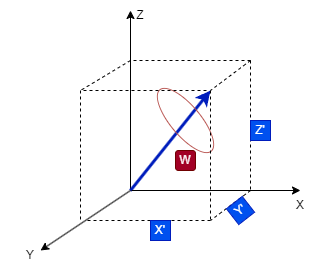
\includegraphics[width=70mm, keepaspectratio]{figures/Diagrammok/Quaterion}
\caption{Quaterion térvektor által megvalósítható rotáció szemléltetése}
\label{fig:Quaterion}
\end{figure}

Ezzel a módszerrel történő rotációk gyakran alkalmazhatók például térbeli orientációk számítására a robotika területén. A rotációkat általában egy kezdeti orientáció és egy célorientáció közötti kvaternióként reprezentálják, majd ezeket a kvaterniókat alkalmazzák a térbeli objektumokon. Fontos megjegyezni, hogy a quaternionok bevezetése és használata egy speciális terület a matematikában, és gyakran igényel némi megértést a térgeometriában és lineáris algebrában.

\section{Gazebo szimuláció}
%----------------------------------------------------------------------------

A célkitűzésem egyike az volt, hogy a telemanipulátorral szimulációs környezetben tudjak vezérelni egy robot kart. Ezt azért tartom nagyon fontos lépcsőfoknak a valós robot vezérlést megelőzően, mert kvázi előellenőrzése az elkészített rendszernek. Bármilyen súlyos matematikai hiba vagy súlyos anomália, ami veszélyeztetné a robot épségét szimulációnál jelentkezni fog. A szimulációt Gazebo-val készítettem és teszteltem. Ugyanazt a hardvert használtam amin később a valós robot vezérlést is végeztem, így sikerült meggyőződnöm arról, hogy a hardver és a szoftveres rendszer is megfelelően működik. A szimulációs robot vezérlés sikerült és egy Universal Robot 5-ös típusú robotot az elvárásoknak megfelelően sikerült vezérelni szimulációs környezetben.

A szimulációs rendszerek alapvető tulajdonsága, hogy azt szimulálják le, ami fel van nekik programozva. Ezeket a szimulációs elemeket a teljesség igénye mellett se lehet egy az egyeben megfeleltetni a valós életben megtalálható igazinak. Ebből fakadólag előfordulhatnak pálya tervezési hibák, zajok és olyan előre nem lekezelt program futásbeli hibák, amik a programok rossz időbeli sorrendje miatt keletkeznek. Ezeket a problémákat jellemzően a szimulációs rendszer korlátainak tekintjük. Az általam futtatott szimulációnál, csak azokra a tapasztalatokra térek ki, amik közvetlenül a telemanipulátor, a kontroller és a robotvezérlő működésével kapcsolatos. A tapasztalatokat összegzem és a valós robot vezérlésénél össze is fogom hasonlítani.

%TODO Kép a szimulációról

Egy meghatározott cél koordináta és a jelenlegi között nincs nagy távolság, akkor gyorsan végrehajtja a parancsot. Nagy távolság esetén a számítási idő szignifikánsan nagyobb. Ez akár egyértelmű is lehet viszont, egy nagyon nagy hátrány, mert nem is feltétlen a TCP pontok távolsága számít, hanem az az egyenlet rendszer, aminek eredményeként a lehetséges orientációkat megkapjuk. Ezzel kapcsolatosan megfigyeltem még, hogy a nagyon összetett pályák esetén még a $5[s]$-os időtúllépést is elérheti kontroller, amikor is a számítás kiáll hibára és megszakítja a kalkulációt. Ezt követően vagy visszatér és egy következő orientációt kezd el számolni, vagy helytelen orientáció miatt beavatkozást igényel a szimulátor. Amit még a valós robot szimulációval való korrekt összehasonlítás miatt fontos volt megfigyelnem, hogy stabil egy adott pontban, nem érzékelhető se remegés se bizonytalan pozíciótartás.

A szimulációs tesztelés sikeres volt. Ez a megközelítés a későbbiekben is hasznos lehet, ha új funkciók implementálódik vagy modul csere történik a rendszerben. Így mindent nagy vonalakban lelehet tesztelni mielőtt valós roboton elindítanánk.


\section{Valós robot vezérlése}
%----------------------------------------------------------------------------

A diploma dolgozatom végcélja az volt, hogy egy valós robotot is vezéreljek a telemanipulátorommal. 

A robot, amit valójában sikerült mozgatnom, ugyanaz a robot amit a szimulációs környezetben is teszteltem. A robotot laboratóriumi összeállításban teszteltem ezért is látszik, hogy egy sakk tábla van a robot előtt és nem egy témába vágó tárgy (például műtő fatnom), mert a laboratóriumi körülmények között más kollégák is használták. A laboratóriumban a szimuláció és a valós vezérlés közti alapvető különbségekre voltam kíváncsi.

%TODO Kép a robot

Az egyértelműen kijelenthető, hogy sikerült a robotot vezérelni és közel azonos tapasztalatokat gyűjtöttem, mint a szimuláció esetében. A tervezési idő erősen függ a kezdő és végpont távolságától, illetve ugyanúgy időtúllépéssel leáll mint a szimuláció esetében. Lényeges különbség viszont, hogy nagyon látványosan megjelenik egy nyugvó pont körüli zaj. A robot kismértékben remeg/mozog olyankor amikor a telemanipulátor által a vezérlő nem ad direktben mozgásutasítást. Ez nagyon nagy rendszer hiba, mivel a sebészeti szimulációk vagy későbbiekben műtő fantom operálására szeretném tovább fejleszteni, akkor ez mozgás megengedhetetlen, de ezt a következő fejezetben részletesebben bemutatom.

A valós robot mozgatással sikeresnek tekintettem a fejlesztésnek ezt a szakaszát. Az elképzelésemet meg lehet valósítani, ennek a pontosítását már további munkával lehet javítani. 

\section{Koncepcionális hibák}

Az előző fejezetben a robot mozgatásnál tapasztalt bizonytalan mozgásnak és remegésnek több oka lehet, amelyek közül néhány ismert a számomra.

A mikrovezérlőtől indulva a szenzorok jele a feldolgozás során a gyártó által jelezve is $1^\circ$-os hibával működhet. Például, ha ez az első csuklóban jelenik meg, a példa kedvéért pozitív irányban, akkor a end-effektor $x$ vagy $y$ irányban közel $6[mm]$-t is tévedhet, ami elfogadatlan. Egyértelműen ilyen nagy mértékű hiba nagyon szélsőséges esetben jelenhet meg, viszont kisebb szöghibák a hat csuklón halmozottan okozhatnak bármelyik tengelyen hasonló nagyságrendű hibát. A szöghiba zajszűrésére lehetőség van, de nagyon körül tekintően kell eljárni, mivel a GMR szenzorok előnye pont abban van, hogy érzékenyek a kis mágneses tér változásra. A legegyszerűbb, de nem a legolcsóbb lehetőség, ha redundánsan csuklónkként egy pár szenzort használok ezzel akár átlagolás, akár felülbírálói megoldással tudom csökkenteni a hibát.

A zajnak a másik oka szintén ebből a szöghibából adódik, de a kontrollerben nem elnyomódik, hanem felerősödik. Ennek nem fizikai, hanem matematikai oka van, ugyanis a kinematikai számítások összetettsége miatt több kerekítés lehet a számítások során. A kerekítések nem feltétlen a számítási kapacitás hiánya miatt, hanem a vezérelni kívánt robot ismétlési pontossága miatt is lehetséges. A UR 5 ismétlési pontossága a gyári adatok alapján $0,1[mm]$ és $0,03[mm]$ között lehet. Azt, hogy a remegés emiatt lenne érezhető a robotkarban kevésbé tartom valószínűnek. Arra, hogy a remegés mi miatt jön létre a robotban mindenképpen szeretnék választ találni.